\section{Experiments}
\subsection{Data Source}
We perform the researcher future citation prediction on the Google Scholar database.
It covers 3,666,012 publications by 23,140 researchers for more than 50 years.
The total number of citations is 128,157,386 in this data set.

We used all papers with cross validation to formulate the publication level future citation prediction model.
With this model we created a new feature that aggregates all the number of citation predicted from all papers a researcher published before year $t$.

For each researcher who has been active for at least $\Delta t$ years, we generate a new record in a new data set for each year after the first $\Delta t$ years, i.e. if a researcher has been active for 40 years and $\Delta t=5$. 35 records are generated for every year after five years in the field. 

We first clean all records with an N/A value by removing the entire row.
We split the entire data set randomly into two parts, $80\%$ for training and validation and $20\%$ for test.
For the $80\%$ data, we split it into two parts. $75\%$ are used for training and $25\%$ are used for validation.
We select the best hyper parameter using training set and validation set. We then used the best hyper parameter to train a model on both training set and validation set. Finally, we test our model on the test set.

We compare our predicted future citations with actual future citations in the test set.

\subsection{Evaluation}
The coefficient of determination ($R^2$) is used in evaluating how well prediction model fits the test data. Let the set of all researchers be $R$, then the definition of $R^2$ is:
\[R^2=\frac{\sum_{r \in R}(\hat{D_c}(r,t,\Delta t)-f(r|\vec{X},t,\Delta t))^2}{\sum_{r \in R}(\hat{D_c}(r,t,\Delta t)-\bar{D_c}(r,t,\Delta t))^2}\]
where $\hat{D_c}$ is the actual future citation for researcher $r$ in year $t$, $f$ is our prediction
and $\bar{D_c}$ represents the mean of the actual citations from year $t$ to $t+\Delta t$ for all researchers.

By definition, $R^2 \leq 1$, with $R^2=0$ means the predicted citations does not fit the actual citations at all,
and $R^2=1$ means the model perfectly predicted the future citations. A model with a larger $R^2$ indicates a better prediction performance and is therefore desired. 
\subsection{Prediction Performance}
Following Yan et al.'s work, our prediction model for publication future citation is summarized in table \ref{tbl-pubprediction}.

\begin{table}[!h]
\begin{center}
\begin{tabular}{c|c|c|c|c|c}
\hline
$R^2$& LR & DFR & PR & LASSO & Ridge\\
\hline
$\Delta t=1$ & & & & &\\
\hline
$\Delta t=5$ & & & & &\\
\hline
$\Delta t=10$ & & & & &\\
\hline
\end{tabular}
\end{center}
\caption{Publication future citation prediction evaluation}
\label{tbl-pubprediction}

\end{table}

We achieved a much better regression result by performing a data cleaning and using decision forest regression as our model. We then use the trained model to compute the predicted publication future citation counts. Finally, for each author and year, we sum the number of predictions from publication future citation counts prediction as a new feature we discussed above.

The prediction for researcher future citations is summarized in table \ref{tbl-r2}.
The best predictive performance for next five year researcher citations is plotted in figure \ref{author-prediction}.


\begin{figure}
    \centering
    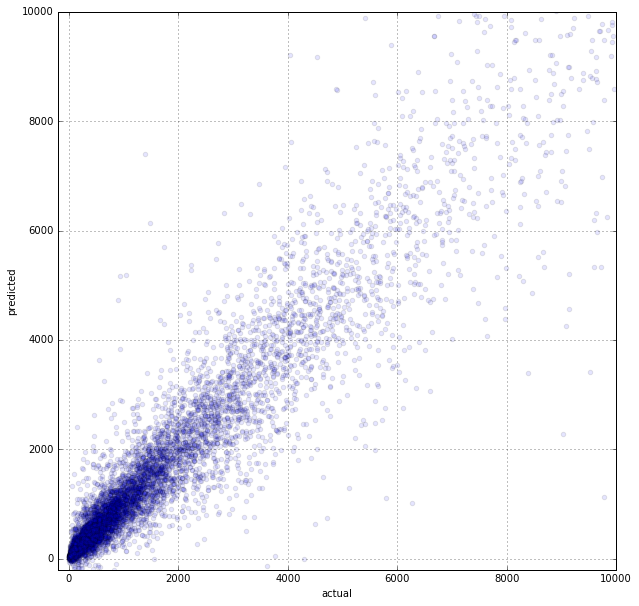
\includegraphics[width=\columnwidth]{fig/author-prediction.png}
    \caption{Author Citations in Next 5 Years, Prediction vs. Actual.}
    \label{author-prediction}
\end{figure}

\begin{table*}[t]
\begin{center}
\begin{tabular}{c|c|c|c|c|c|c|c|c|c|c|c|c|c|c|c}
\hline
& \multicolumn{5}{|c|}{\textbf{$\Delta t =1$}}& \multicolumn{5}{|c|}{$\Delta t =5$}& \multicolumn{5}{|c}{$\Delta t =10$}\\

\hline
Methods & LR & DFR & PR & SVR & R& LR & DFR & PR & SVR & R& LR & DFR & PR & SVR & R\\
\hline\hline
+org.Rank & & & & & & & & & & & & & & & \\
\hline
+$N_c(r,t)$ & & & & & & & & & & & & & & & \\
\hline
+index & & & & & & & & & & & & & & & \\
\hline
+years & & & & & & & & & & & & & & & \\
\hline\hline
-org.Rank & & & & & & & & & & & & & & & \\
\hline
-$N_c(r,t)$ & & & & & & & & & & & & & & & \\
\hline
-index & & & & & & & & & & & & & & & \\
\hline
-years & & & & & & & & & & & & & & & \\
\hline\hline
Combined & & & & & & & & & & & & & & & \\
\hline
\end{tabular}
\end{center}
\caption{The performance of various predictive models on the test set."+""-"}
\label{tbl-r2}

\end{table*}



\subsubsection{Citation Distribution}
As is shown in figure \ref{author-prediction}, the distribution of future researchers citations shows a long tail. 
Most researchers gets a total future citations less than 2,500 cites.
However, even with this long tail distribution, our publication level feature leveages this problem and achieved an overall $R^2$ at $0.957$.

\subsubsection{Factor Contribution}
As we shall see in table \ref{tbl-r2}, three major factors that have a strong impact on the prediction performance are historical citation counts, indexes that represent the performance of research performance and the publication level feature that we introduced before.

Since we are prediction the number of future citation counts of a researcher, both historical yearly citation counts and historical total citation counts are useful features. A simple linear combination of these features forms a good representation of the future citation counts. It is trivial that these historical citation counts feature contributes a big improvement on prediciton performance.

H-index and i-10 index as have been discussed in the previous section will have a good representation on the research performance. Hirsh states that h index has a better prediction property to total citation counts\cite{Hirsh2007does}. However, since we are predicting the future citation counts which is the difference of citation counts between now and the future, H-index and i-10 index are relatively a weaker indicator compared to the historical citation counts.

Our unique feature, the publication level prediction helps improve the prediction performance from $R^2 = 0.750$ to $R^2 = 0.957$ using decision forest regression method. The feature itself can predict the citation count in the next 5 years as good as historical citations. Both the publication level prediction and historical citations performs better than h-index and i10-index combined.
